% !TEX encoding = UTF-8 Unicode

\documentclass[a4paper]{article}

\usepackage{color}
\usepackage{url}
\usepackage[T2A]{fontenc} % enable Cyrillic fonts
\usepackage[utf8]{inputenc} % make weird characters work
\usepackage{graphicx}
\usepackage[verbatim]

\usepackage[english,serbian]{babel}
%\usepackage[english,serbianc]{babel} %ukljuciti babel sa ovim opcijama, umesto gornjim, ukoliko se koristi cirilica

\usepackage[unicode]{hyperref}
\hypersetup{colorlinks,citecolor=green,filecolor=green,linkcolor=blue,urlcolor=blue}

%\newtheorem{primer}{Пример}[section] %ćirilični primer
\newtheorem{primer}{Primer}[section]

\usepackage{listings}
\definecolor{mygreen}{rgb}{0,0.6,0}
\definecolor{mygray}{rgb}{0.5,0.5,0.5}
\definecolor{mymauve}{rgb}{0.58,0,0.82}

\lstset{ 
	backgroundcolor=\color{white},   % choose the background color; you must add \usepackage{color} or \usepackage{xcolor}; should come as last argument
	basicstyle=\scriptsize\ttfamily,        % the size of the fonts that are used for the code
	breakatwhitespace=false,         % sets if automatic breaks should only happen at whitespace
	breaklines=true,                 % sets automatic line breaking
	captionpos=b,                    % sets the caption-position to bottom
	commentstyle=\color{mygreen},    % comment style
	deletekeywords={...},            % if you want to delete keywords from the given language
	escapeinside={\%*}{*)},          % if you want to add LaTeX within your code
	extendedchars=true,              % lets you use non-ASCII characters; for 8-bits encodings only, does not work with UTF-8
	firstnumber=1000,                % start line enumeration with line 1000
	frame=single,	                   % adds a frame around the code
	keepspaces=true,                 % keeps spaces in text, useful for keeping indentation of code (possibly needs columns=flexible)
	keywordstyle=\color{blue},       % keyword style
	language=Python,                 % the language of the code
	morekeywords={*,...},            % if you want to add more keywords to the set
	numbers=left,                    % where to put the line-numbers; possible values are (none, left, right)
	numbersep=5pt,                   % how far the line-numbers are from the code
	numberstyle=\tiny\color{mygray}, % the style that is used for the line-numbers
	rulecolor=\color{black},         % if not set, the frame-color may be changed on line-breaks within not-black text (e.g. comments (green here))
	showspaces=false,                % show spaces everywhere adding particular underscores; it overrides 'showstringspaces'
	showstringspaces=false,          % underline spaces within strings only
	showtabs=false,                  % show tabs within strings adding particular underscores
	stepnumber=2,                    % the step between two line-numbers. If it's 1, each line will be numbered
	stringstyle=\color{mymauve},     % string literal style
	tabsize=2,	                   % sets default tabsize to 2 spaces
	title=\lstname                   % show the filename of files included with \lstinputlisting; also try caption instead of title
}

\begin{document}
	
	\title{Analiza projekta korišćenjem alata za verifikaciju softvera\\ \small{Seminarski rad u okviru kursa\\Verifikacija softvera\\ Matematički fakultet}}
	
	\author{Milica Karličić, 1002/2022\\ milicakarlicic1801@gmail.com}
	\date{januar 2023.}
	\maketitle
	
	\abstract{
		U ovom radu biće opisana detaljna analiza projekta \textit{Fire and Water}. U daljem tekstu biće ukratko opisani alati i naredbe koji su korišćeni prilikom analize. Svaka glava sadrži pronađene greške ili određene statističke podatke vezane za dati projekat. Na samom kraju opisa rada i analize pojedinih alata mogu se naći i načini na koji bi pronađene greške mogle da se otklone. 
 	}
	
	\tableofcontents
	
	\newpage
	
	\section{Uvod}
	\label{sec:uvod}
	Projekat \textit{Fire and Water} predstavlja jednu implementaciju popularne istoimene igrice. Igrica prati dva glavna igrača $waterGirl$ i $fireBoy$ čiji je cilj da sakupe što više dijamanata i da, izbjegavajući prepreke, stignu do cilja. Za testiranje projekta \textit{Fire and Water} korišćeni su alati za dinamičku i statičku analizu. Za dinamičku analizu projekta korišćeni su $Valgrind$ i $Perf$. Izvještaj statičke analize dobijen je na osnovu rada alata \textit{Clang-Tidy}, $Clazy$ i $Clangd$. Alati za dinamičku analizu su pozivani iz komandne linije, dok se za alate statičke analize koristila podrška $Qt$ razvojnog okruženja.
	
	\section{Valgrind}
	$Valgrind$ je profajler otvorenog koda koji nadgleda rad željenog programa i prijavljuje nepravilnosti u radu programa. Valgrind distribucija sadrži naredne alate:
	\begin{itemize}
		\item $Memcheck$ - detektor memorijskih grešaka
		\item $Massif$ - praćenje rada dinamičke memorije
		\item $Cachegrind$ - profajler keš memorije
		\item $Callgrind$ - profajler funkcija
		\item $Helgrind$ i $DRD$ - detektor grešaka niti
	\end{itemize} \cite{verifikacija1}
	
Alati $Valgrinda$ koriste metodu bojenja vrijednosti. Oni svaki registar i memorijsku vrijednost boje (zamjenjuju) sa vrijednošću koja govori nešto dodatno o originalnoj vrijednosti. Proces rada svakog alata $Valgrinda$ je u osnovi isti. U ovom radu biće prikazana upotreba alata $Memcheck$ i $Cachegrind$. \cite{verifikacija2}

Zbog velikog usporenja prilikom izvršavanja programa upotrebom Valgrind-a napravljena je druga verzija projekta koja je jednostavnija za analizu. Naime, kako je cilj testirati studentski kod, Qt biblioteke bi mogle da se izbace što samim tim podrazumijeva uklanjanje određenih klasa i metoda. U modifikovanom projektu sadržaj $main$-a prikazan je na \ref{fig:main}.

	\begin{figure}[h!]
		\centering
		\caption{$Main$ modifikovanog projekta}
		\label{fig:main}
		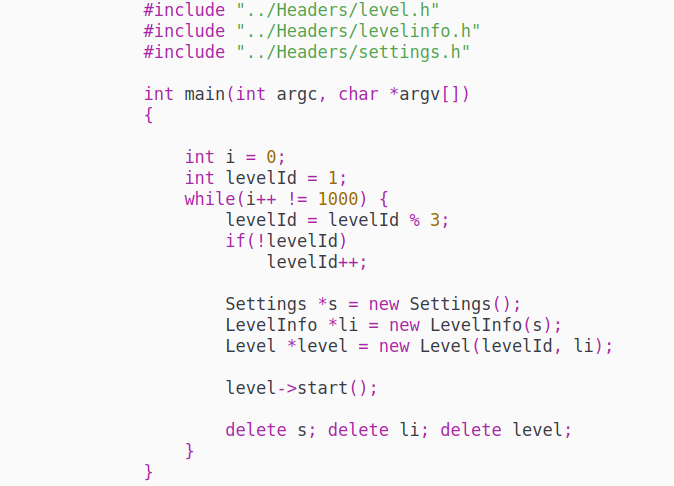
\includegraphics[scale=0.5]{main1.png}
	\end{figure}

	\subsection{Memcheck}
	Prilikom analize $Qt$ projekta, $Memcheck$ se može pozivati iz $QtCreator$-a ili korišćenjem komandne linije. U ovom radu biće simulirana upotreba alata iz terminala. 
	
Greške koje mogu biti detektovane upotrebom $Memcheck$ alata su:
\begin{itemize}
	\item Korišćenje nedefinisanih vrednosti
	\item Čitanje ili pisanje u nedopuštenu memoriju na hipu, steku
	\item Neispravno oslobađanje memorije na hipu
	\item Poklapanje argumenata src i dest funkcije memcpy i njoj sličnim
	\item Prosleđivanje loših vrednosti za veličinu memorijskog prostora funkcijama za alokaciju memorije, npr. negativnih.
	\item Curenje memorije, npr. gubitak pokazivača na alociran prostor.
\end{itemize}

Na osnovu prethodno pomenutog $main$-a $Memcheck$ je detektovao curenje memorije na nekoliko mjesta. U okviru $makefile$-a veoma je važno proslijediti kompajleru g++ opcije -g -O0 kako bi se kod preveo sa debug simbolima i bez optimizacija tj. kako bismo imali uvid u tačan redni broj linije koda u kojoj je došlo do neke greške (u našem slučaju u pitanju je curenje memorije). Opcije koje ćemo koristiti prilikom poziva Memcheck alata su --leak-check=full i --show-leak-kinds=all koje nam prikazuju detaljan opis pronađenih curenja memorije. Pozivom programa sa valgrind --leak-check=full --show-leak-kinds=all $./a.out$ dobijamo izlaz prikazan na slikama \ref{fig:mem1} i \ref{fig:mem2}.

\begin{verbatim}
	
\end{verbatim}

	\begin{figure}[h!]
		\caption{$Memcheck$}
		\label{fig:mem1}
		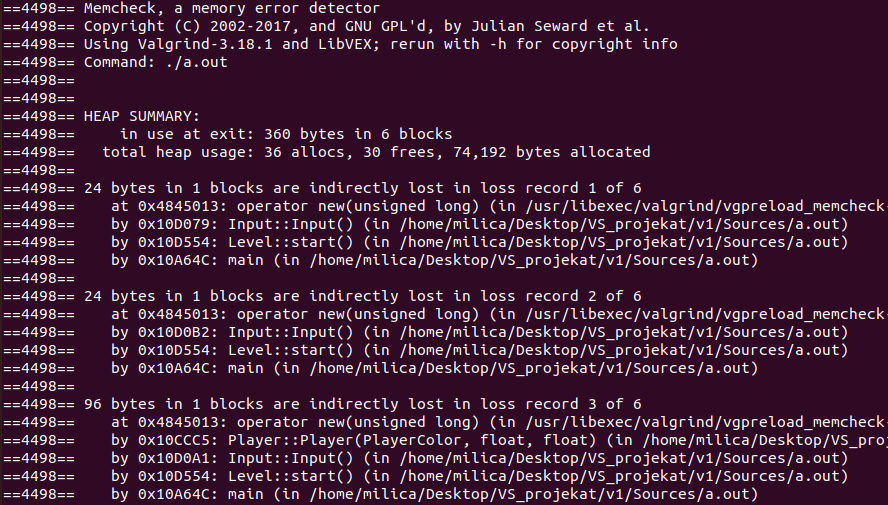
\includegraphics[scale=0.5]{mem1.png}
	\end{figure}
	\begin{figure}[h!]
		\caption{$Memcheck$}
		\label{fig:mem2}
		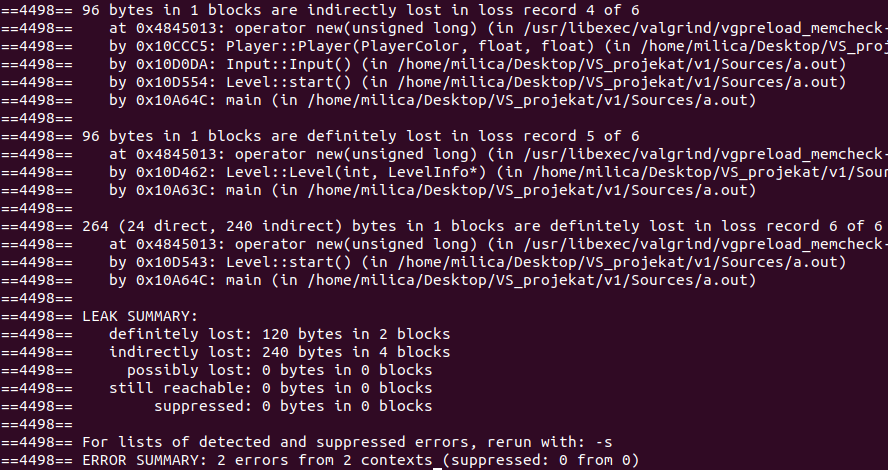
\includegraphics[scale=0.5]{mem2.png}
	\end{figure}
	
Na osnovu rezultata možemo vidjeti prisustvo curenja memorije na šest mjesta u programu. Detektovana curenja memorije su sledeća:
\begin{itemize}
	\item {u klasi player.cpp:
	\begin{itemize}
		\item Linija 12: inicijalizovana promenljiva info se nikada ne oslobađa (greška se javlja dva puta, jednom prilikom inicijalizacije vatrenog igrača, a drugi put prilikom inicijalizacije vodenog igrača)
	\end{itemize}}
	
	\item {u klasi input.cpp:
	\begin{itemize}
		\item Linija 23: objekat koji odgovara vatrenom igraču se nikada ne oslobađa
		\item Linija 24: objekat koji odgovara vodenom igraču se nikada ne oslobađa
	\end{itemize}}
	
	\item {u klasi level.cpp:
	\begin{itemize}
		\item Linija 36: inicijalizovana promenljiva info se nikada ne oslobađa
		\item Linija 51: inicijalizovana promenljiva input se nikada ne oslobađa
	\end{itemize}}
\end{itemize}
Na osnovu izvještaja možemo vidjeti da se poslednja dva curenja odnose na direktno izgubljene blokove tj. na promenljive info i input iz start() metode klase level.cpp. Direktno izgubljeni blokovi mogu povlačiti gubitak i nekih drugih blokova koji u tom slučaju postaju indirektno izgubljeni. Indirektno izgubljeni objekti u ovom primjeru su: promenljive info iz klase player.cpp i promenljive koja odgovara vatrenom odnosno vodenom igraču iz klase input.cpp.

Kako je analiza rađena na modifikovanoj verziji projekta neophodno je provjeriti da li su pronađena curenja prisutna i u originalnoj verziji. Jednostavnim pregledom klasa se potvrđuje prisustvo svih navedenih grešaka i u originalnom kodu, što je i očekivano.
U originalnom projektu moguće je curenje memorije i na nekim drugim mjestima koja su vezana za GUI aplikacije.


	\subsection{Cachegrind}
	Prilikom analize $Qt$ projekta, $Memcheck$ se može pozivati iz $Qt$ $Creator$-a ili korišćenjem komandne linije. U ovom radu biće simulirana upotreba alata iz terminala. 
Cachegrind je alat Valgrind-a koji omogućava softversko profajliranje keš memorije tako što simulira i prati pristup keš memoriji mašine na kojoj se program, koji se analizira, izvršava. Takođe, može se koristiti i za profajliranje izvršavanja grana.  \cite{verifikacija1}
Cachegrind simulira memoriju mašine, koja ima prvi nivo keš L1 memorije podeljene u dve odvojene nezavisne sekcije: I1 - sekcija keš memorije u koju se smeštaju instrukcije D1 - sekcija keš memorije u koju se smeštaju podaci. Drugi nivo keš memorije koju Cachegrind simulira je objedinjen - LL, skraćeno od eng. last level. Ovaj način konfiguracije odgovara mnogim modernim mašinama. \cite{verifikacija2}
U okviru $makefile$-a veoma je važno da  kompajleru g++ ne proslijedimo opciju  -O0 tj. sasvim je u redu da vršimo analizu optimizovanog koda jer želimo da testiramo program u njegovom normalnom izvršavanju. Pozivom programa sa valgrind --tool=cachegrind $./a.out$ dobijamo izlaz prikazan na slici \ref{fig:cache1}.
	\begin{figure}[h!]
		\caption{$Cachegrind$ - izlaz prilikom jednog izvršavanja petlje}
		\label{fig:cache1}
		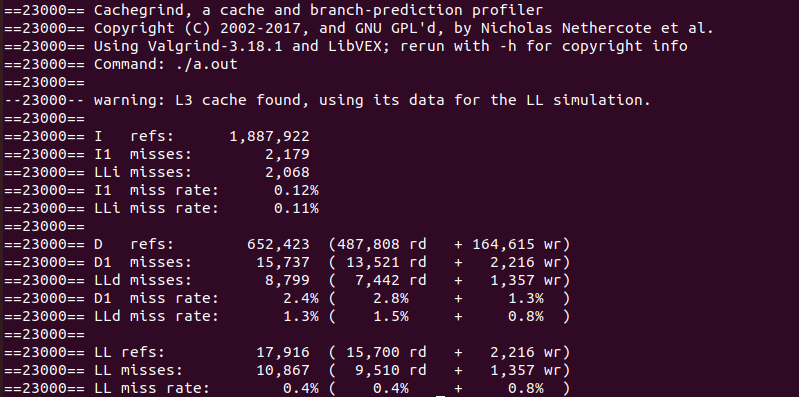
\includegraphics[scale=0.5]{cache1.png}
	\end{figure}

Dobijeno upozorenje je u vezi sa radom $Cachegrind$-a. Naime, kao što je već rečeno $Cachegrind$ radi sa dva nivoa cache memorije dok su na arhitekturi koja se koristi za testiranje prisutna tri nivoa. To nije toliko bitno, samo označava da je moguće da će se program brže izvršavati na datoj arhitekturi.
Ukoliko u $main.cpp$ broj iteracija povećamo na 1000, dobijamo izlaz prikazan na slici \ref{fig:cache2}.
	\begin{figure}[h!]
		\caption{$Cachegrind$ - izlaz prilikom povećavanja iteracija petlje}
		\label{fig:cache2}
		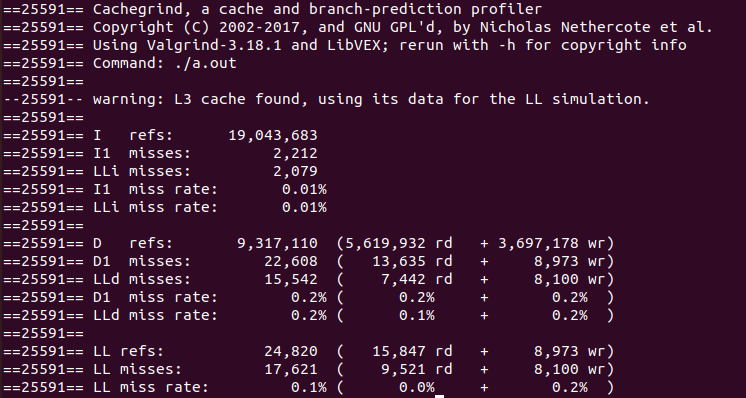
\includegraphics[scale=0.5]{cache2.png}
	\end{figure}

Na osnovu ovog i prethodnog primjera možemo vidjeti da se broj promašaja keša za instrukcije i podatke značajno smanjio. Takođe, možemo vidjeti da se u prvom slučaju skoro tri puta više pristupalo kešu sa instrukcijama nego kešu sa podacima, dok se u drugom slučaju taj broj smanjio na dva. 

Detaljniji izvještaj $Cachegrind$-a nalazi se u fajlovima \textit{cachegrind.out.<PID>} čiji sadržaj možemo ispisati komandom \textit{cg\_annotate}. Na samom početku datog fajla možemo pročitati neke karakteristike keš memorija koje se koriste što se može vidjeti na slici \ref{fig:cache3}.
	\begin{figure}[h!]
		\centering
		\caption{$Cachegrind$ - osnovne karakteristike keša}
		\label{fig:cache3}
		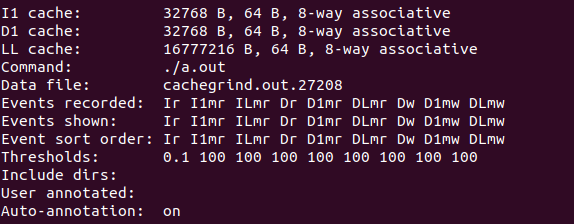
\includegraphics[scale=0.6]{cache3.png}
	\end{figure}

Prvi broj predstavlja veličinu keša, drugi broj predstavlja veličinu linije (u keš pišemo liniju po liniju) dok treći predstavlja asocijativnost keša. Prilikom pozivanja alata $Cachegrind$ moguće je da promijenimo veličinu $LL$ keša. Ukoliko povećamo veličinu linije na $128$ dobijamo izlaz koji se može vidjeti na slici \ref{fig:cache4}.
	\begin{figure}[h!]
		\centering
		\caption{$Cachegrind$ - promjena veličine linije $LL$ keša}
		\label{fig:cache4}
		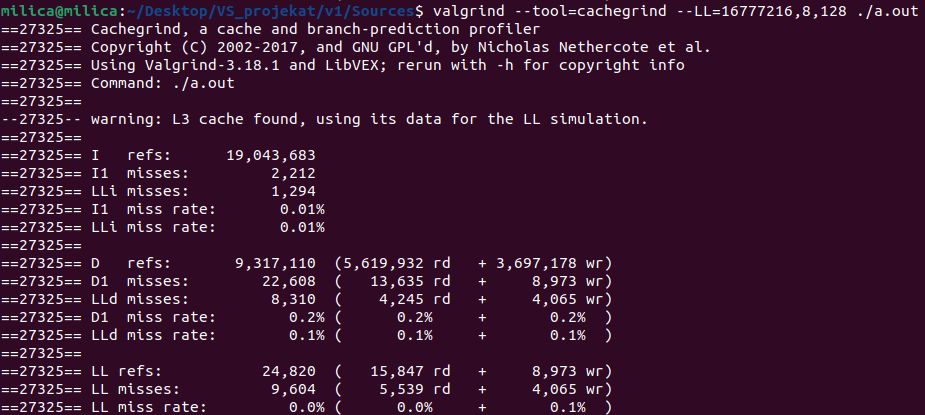
\includegraphics[scale=0.4]{cache4.png}
	\end{figure}
	
Dakle, vidimo da se broj promašaja $LL$ keša smanjio skoro duplo, što je i očekivano s obzirom na to da je veličina linije duplo povećana.
Sa druge strane, ako povećamo veličinu $LL$ keša na \textit{32MB} izlaz $Cachegrind$-a će ostati potpuno isti, tj. u ovom slučaju veličina keša ne utiče na učestalost promašaja \ref{fig:cache5}.
	\begin{figure}[h!]
		\caption{$Cachegrind$ - promjena veličine $LL$ keša}
		\label{fig:cache5}
		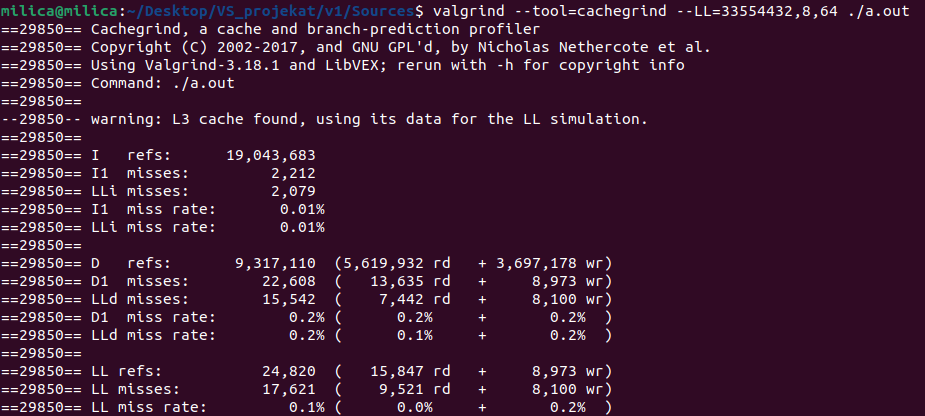
\includegraphics[scale=0.4]{cache5.png}
	\end{figure}

Analiza cachegrind.out.<PID> fajla iz terminala dosta je nepregledna pa se u tu svrhu preporučuje upotreba programa KCachegrind. 

\section{Perf}
	$Perf$ je alat za profajliranje koji pruža jednostavan interfejs preko komandne linije. Zbog brzine rada alata analizu ćemo prikazati nad originalnim projektom (za razliku od $Valgrind$-a za koji smo obrađivali modifikovanu verziju). $Perf$ prikazuje statistike, npr. koliko vremena je provedeno u određenoj funkciji. Profil programa se pravi na osnovu uzorka.
Navedeni alat se može koristiti na dva načina:
\begin{itemize}
	\item kao $Performance$ $Analyzer$ iz $Qt$ $Creator$ okruženja
	\item iz komandne linije
\end{itemize}
Upotreba $Perf$-a iz $Qt$ $Creator$-a je jednostavna: pokretanjem $Performance$ $Analyzer$-a u okviru debug prozora biće prikazane statistike vezane za sam projekat. Ukoliko ipak želimo da koristimo $Perf$ iz komandne linije koristimo sledeće naredbe:
\begin{itemize}
	\item izgraditi $Qt$ projekat
	\item pozicionirati se u $build$ folder
	\item perf record --call-graph dwarf ./FireAndWater
	\item perf report
\end{itemize}

	\begin{figure}[h!]
		\caption{\textit{Perf} - izvještaj}
		\label{fig:p1}
		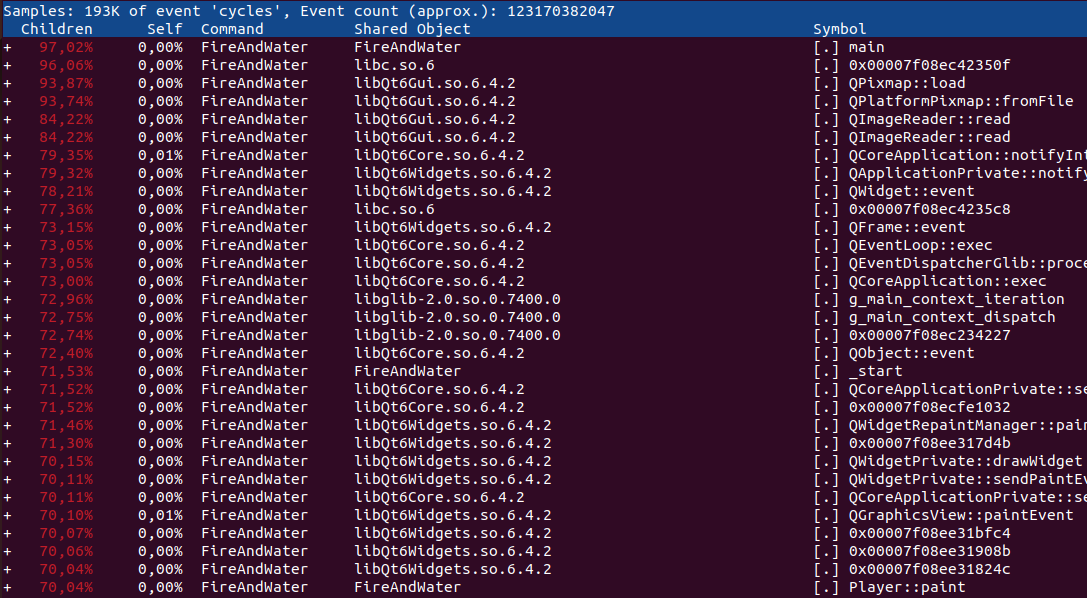
\includegraphics[scale=0.4]{p1.png}
	\end{figure}
	
	Na slici \ref{fig:p1} možemo vidjeti rezultat $Perf$ izvještaja. Kolona $self$ predstavlja procentualno izvršavanje funkcije na osnovu izabranog uzorka. Zbir kolone self treba da bude 100\%. Za funkciju g kažemo da je dijete funkcije f ukoliko postoji konačan niz funkcija $f_1,...,f_n$ $n>=0$ tako da $f \rightarrow f_1\rightarrow...\rightarrow f_n\rightarrow g$ ($a \rightarrow b$ u značenju funkcija a poziva funkciju b). U koloni $children$ prikazano je procentualno izvršavanje sve djece navedene funkcije. Kako pokrećemo igricu iz $main$-a to je očekivano da će broj izvršavanje njene djece biti najveći. 
	
Za vizuelizaciju podataka dobijenih naredbom $perf$ $report$ koristićemo tzv. vatreni dijagram \ref{fig:p2}. Dijagram prikazuje populaciju uzoraka na $x$ osi a dubinu steka na $y$ osi. Svaka funkcija je jedan pravougaonik, širine relativne broju uzoraka. Vatreni dijagram se može dobiti na sledeći način:
\begin{itemize}
	\item git clone --depth 1 https://github.com/brendangregg/FlameGraph
	\item cp ../perf.data ./
	\item perf script | ./stackcollapse-perf.pl | ./flamegraph.pl > perf.svg
	\item Firefox perf.svg
\end{itemize}
	
	\begin{figure}[h!]
		\caption{\textit{Perf} - vatreni dijagram}
		\label{fig:p2}
		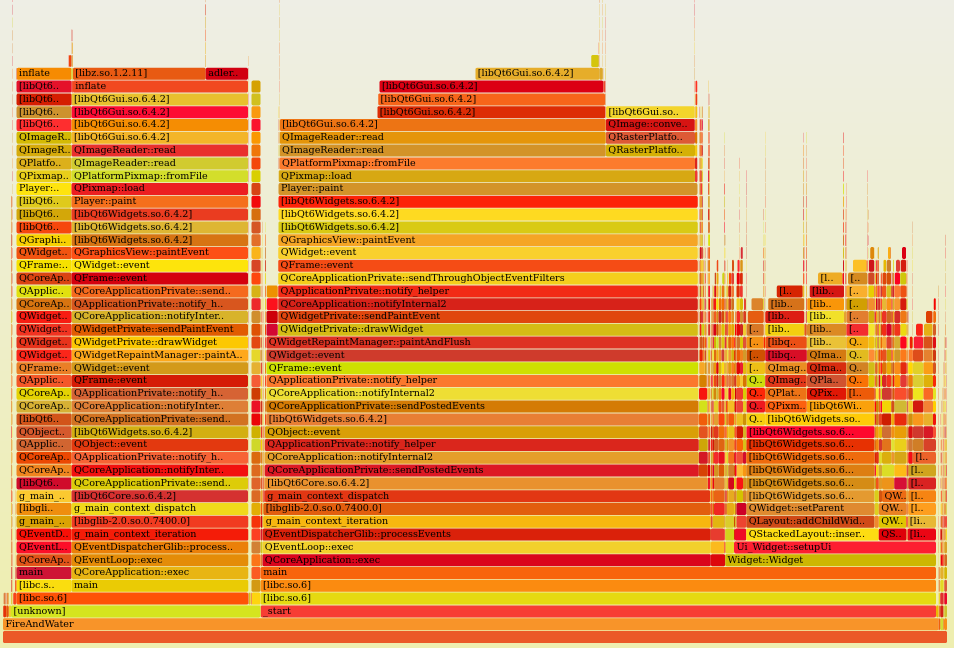
\includegraphics[scale=0.4]{p2.png}
	\end{figure}

Na grafiku pored velikog broja $Qt$ funkcija možemo uočiti i neke poznate funkcije i metode kao što su $main$, \textit{Widget::widget}, \textit{Player::paint}. Vodeći se datim statistikama, najviše napora za optimizaciju treba uložiti upravo u prethodne navedene funkcije, iz razloga što se najčešće izvršavaju. Nakon otvaranja vatrenog grafika u $browser$-u možemo vidjeti iskorišćenje $CPU$-a na osnovu broja uzoraka koji su korišćeni.

\section{Clang-Tidy i Clazy}
	U okviru $Qt$ $Creator$-a postoje ugrađeni alati \textit{Clang-Tidy} i $Clazy$ koji za detektovanje grešaka u programima pisanim u $C$ i \textit{C++} koriste statičku analizu.
\textit{Clang-Tidy} pronalazi standardne programerske greške kao što su nekonzistentnost  u pisanju programa i greške u radu sa interfejsima. Statički analizator $Clang$ je dio \textit{Clang-Tidy}.
$Clazy$ omogućava $Clang$-u da razumije semantiku $Qt$-a. $Clazy$ prikazuje upozorenja kompajlera vezana za $Qt$, u rasponu od nepotrebne alokacije memorije do zloupotrebe $API$-ja i pruža akcije za rešavanje nekih problema.
Upotreba \textit{Clang-Tidy} i $Clazy$ iz $Qt$ $Creator$-a (kao i ostalih analizatora koji su podržani od strane $Qt$ $Creator$-a) se svodi na sledeće:

\begin{itemize}
	\item U okviru kartice $Analyze$ odabrati navedene alate \ref{fig:cc1}.
	\begin{figure}
		\centering
		\caption{\textit{\textit{Clang-Tidy} i $Clazy$} - pokretanje}
		\label{fig:cc1}
		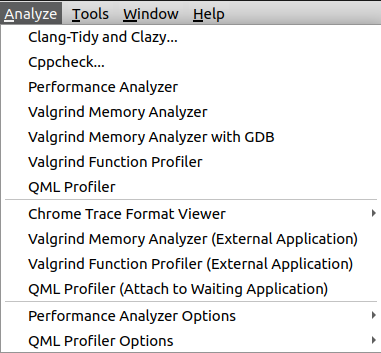
\includegraphics[scale=0.4]{cc1.png}
	\end{figure}
	\item Označavanje fajlova koje želimo da testiramo. Zbog brzine analizatora i kompletnosti provjere preporučuje se analiza svih dostupnih fajlova u okviru projekta \ref{fig:cc2}.
	\begin{figure}[h!]
		\centering
		\caption{\textit{\textit{Clang-Tidy} i $Clazy$} - podešavanje}
		\label{fig:cc2}
		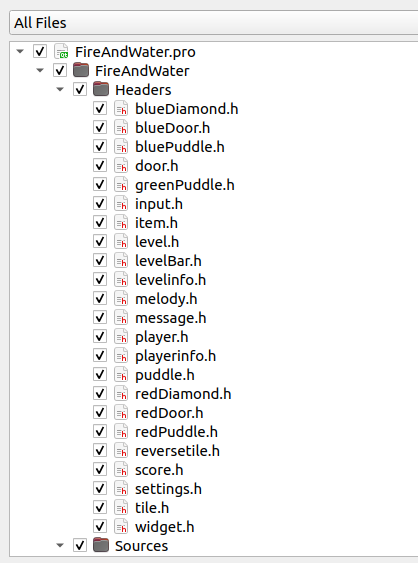
\includegraphics[scale=0.4]{cc2.png}
	\end{figure}
\end{itemize}

Pokretanjem alata \textit{Clang-Tidy} i $Clazy$ dobijamo izlaz prikazan na slici \ref{fig:cc3}.
	\begin{figure}[h!]
		\caption{\textit{\textit{Clang-Tidy} i $Clazy$} - rezultat analize programa}
		\label{fig:cc3}
		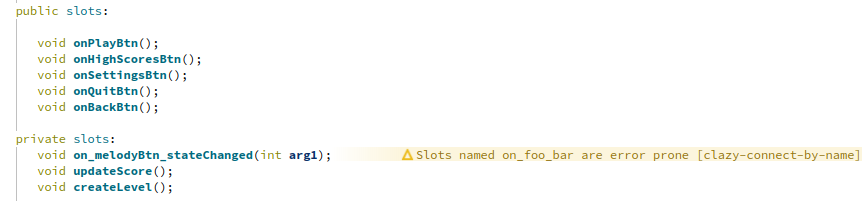
\includegraphics[scale=0.5]{cc3.png}
	\end{figure}
	
	Detektovana greška se odnosi na ime slota (funkcija koja reaguje na signale određenih objekata). Kao što možemo vidjeti na slici, svi slotovi izuzev jednog, koji koristi notaciju sa podvlakom, koriste kamilju notaciju. Zbog osobine konzistentnosti koja je veoma važna prilikom pisanja koda, kako bi se smanjila vjerovatnoća nastanka greške naziv \textit{on\_melodyBtn\_stateChanged} bi trebalo popraviti u \textit{onMelodyBtnStateChanged}.
	
	\section{Clangd}
	
	Clangd je jezički server koji postoji ugrađen u mnogim razvojnim okruženjima. Zasnovan je na $Clang$ $C++$ kompilatoru i dio je $LLVM$ projekta. Koristi se za provjeru ispravnosti koda: ispituje kompletnost, nalazi kompilacione greške, ispituje definicije funkcija… U ovom izvještaju biće prikazana upotreba $Clangd$-a iz $Qt$ $Creator$-a.
Da bismo koristili $Clangd$ neophodno je da podesimo odgovarajuću opciju. U gornjem meniju \textit{Edit->Preferences->C++} i novom prozoru treba označiti opciju \textit{Use clangd} što se može vidjeti na slici \ref{fig:c1}.
	 \begin{figure}[h!]
		\caption{\textit{Clangd} - podešavanja}
		\label{fig:c1}
		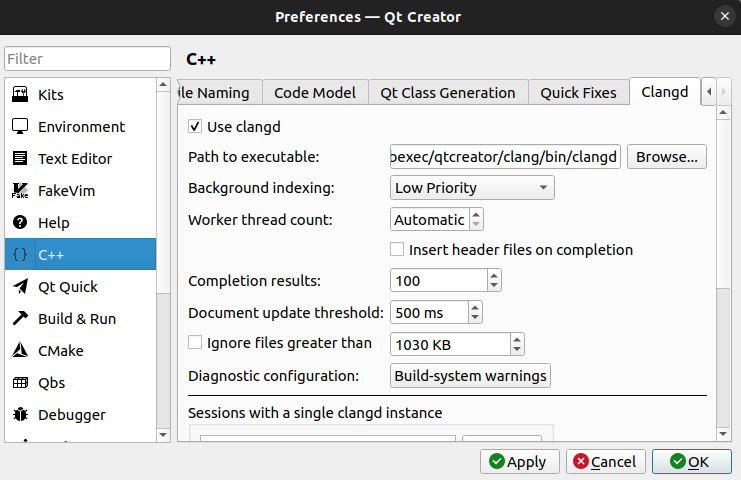
\includegraphics[scale=0.5]{c1.png}
	\end{figure}
	
Nakon toga klikom na $Apply$ i $OK$ biće započeta analiza projekta. Rezultati analize ispitivanog projekta mogu se vidjeti na slici \ref{fig:c2}.
	\begin{figure}[h!]
		\centering
		\caption{\textit{Clangd} - rezultat analize}
		\label{fig:c2}
		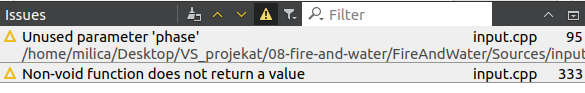
\includegraphics[scale=0.5]{c2.png}
	\end{figure}
	
Dakle, u klasi input.cpp postoji neiskorišćen parametar phase u liniji 95 što možemo vidjeti na slici \ref{fig:c3}.
	\begin{figure}[h!]
		\caption{\textit{Clangd} - neiskorišćen parametar u programu}
		\label{fig:c3}
		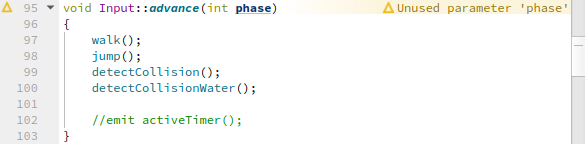
\includegraphics[scale=0.6]{c3.png}
	\end{figure}
Druga pronađena semantička greška je postojanje funkcija koja ne vraća vodi a nema povratnu vrijednost i može se vidjeti na slici \ref{fig:c4}.
	 \begin{figure}[h!]
		\caption{\textit{Clangd} - neispravna povratna vrijednost}
		\label{fig:c4}
		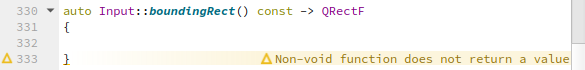
\includegraphics[scale=0.6]{c4.png}
	\end{figure}
	
	U prvom slučaju dovoljno je izbrisati neiskorišćeni parametar a u drugom slučaju, s obzirom na to da je tijelo funkcije prazno, moguće je izbrisati kompletnu deklaraciju kao i definiciju u odgovarajućoj $.hpp$ datoteci. Pronađene greške predstavljaju višak koda u projektu.

\section{Zaključak}
\label{sec:zakljucak}
	
Na samom kraju možemo istaći koliko je primjena alata za verifikaciju važan dio razvoja softvera. Uz jednostavnu primjenu ovih alata u okviru projekta otkrivene greške su curenje memorije, nekonzistentnost i višak koda koje u nekim slučajevima mogu dovesti do fatalnih posledica. Veoma je važno da testiranje radimo što češće prilikom pisanja programa, kako bismo minimizirali vjerovatnoću nastanka grešaka. 
	

\newpage
\addcontentsline{toc}{section}{Literatura}
\appendix
\bibliography{seminarski.bib} 
\bibliographystyle{plain}

	
\end{document}
